% THIS IS SIGPROC-SP.TEX - VERSION 3.1
% WORKS WITH V3.2SP OF ACM_PROC_ARTICLE-SP.CLS
% APRIL 2009
%
% It is an example file showing how to use the 'acm_proc_article-sp.cls' V3.2SP
% LaTeX2e document class file for Conference Proceedings submissions.
% ----------------------------------------------------------------------------------------------------------------
% This .tex file (and associated .cls V3.2SP) *DOES NOT* produce:
%       1) The Permission Statement
%       2) The Conference (location) Info information
%       3) The Copyright Line with ACM data
%       4) Page numbering
% ---------------------------------------------------------------------------------------------------------------
% It is an example which *does* use the .bib file (from which the .bbl file
% is produced).
% REMEMBER HOWEVER: After having produced the .bbl file,
% and prior to final submission,
% you need to 'insert'  your .bbl file into your source .tex file so as to provide
% ONE 'self-contained' source file.
%
% Questions regarding SIGS should be sent to
% Adrienne Griscti ---> griscti@acm.org
%
% Questions/suggestions regarding the guidelines, .tex and .cls files, etc. to
% Gerald Murray ---> murray@hq.acm.org
%
% For tracking purposes - this is V3.1SP - APRIL 2009

\documentclass{acm_proc_article-sp}

\usepackage{color}

%%% still need to break urls

\usepackage[hyphens]{url}


\def\etal{{\it et al.~}}

\newenvironment{packed_enum}{
\begin{enumerate}
  \setlength{\itemsep}{1pt}
  \setlength{\parskip}{0pt}
  \setlength{\parsep}{0pt}
}{\end{enumerate}}

\newenvironment{packed_item}{
\begin{itemize}
  \setlength{\itemsep}{1pt}
  \setlength{\parskip}{0pt}
  \setlength{\parsep}{0pt}
}{\end{itemize}}


\begin{document}



\title{A Survey Wearable Device Risk Perceptions}
%\titlenote{(Does NOT produce the permission block, copyright information nor page numbering). For use with ACM\_PROC\_ARTICLE-SP.CLS. Supported by ACM.}}

%\subtitle{[Extended Abstract]
%\titlenote{Note
%\textit{Note \LaTeX$2_\epsilon$\ and BibTeX} at \texttt{www.website.com}}}


\numberofauthors{1}
\author{
 \alignauthor Linda N. Lee\textsuperscript{1}, Serge Egelman\textsuperscript{1,2}, David Wagner\textsuperscript{1}\\
   \vspace{0.5em}
   \affaddr{\textsuperscript{1}University of California, Berkeley, \{lnl,egelman,daw\}@cs.berkeley.edu}\\
   \affaddr{\textsuperscript{2}International Computer Science Institute, egelman@icsi.berkeley.edu}\\
}

\maketitle



\begin{abstract}
We performed an online survey to examine risk perceptions surrounding wearable computing devices. We controlled for different data types that might be captured, who might have access to that data, and whether it was captured on a wearable device or a smartphone (i.e., to control for familiarity with the technology). We surveyed 1,784 participants about 72 data types, 4 data recipients, and 2 devices to quantify risk perceptions across a wide range of scenarios, along with an evaluation of which factors contribute to the severity of these risks. Following previous work, we also asked participants to perform a risk/benefit analysis comparing 20 new technologies with other well-established technologies. The results of this study can be used to guide future research in wearable device security, especially research that helps to protect sensitive data and guides the design of effective privacy notifications and indicators.
\end{abstract}

% A category with the (minimum) three required fields
\category{K.6.5.}{Management of Computing and Information Systems}{Security and protection}[Unauthorized access]

%\terms{Human Factors}{Measurement}{Security}

\keywords{Privacy, Security, User Studies, Risk Perception, Ubiquitous Computing, Wearables} % NOT required for Proceedings

%%%%%%%%%%%%%%%%%%%
%%%         PAPER BODY         %%%
%%%%%%%%%%%%%%%%%%%


%%%%% FEEDBACK TO INCORPORATE, from Serge

%-"security and privacy concerns regarding wearable devices are becoming heightened as companies make headlines for incidents resulting in users’ sexual activities exposed to the public..." I would rewrite this. You don't really mean to say that tracking sexual activity is the *only* privacy and security concern. It's one of many. I would say at the beginning that there are myriad privacy/security concerns, and then go into specific examples (e.g., sex, facial recognition, etc.).
%-I think you might want to motivate this better: why do we need to better understand the threat landscape? (Answer: to focus on the most concerning things and then warn users when they're about to occur or prevent them from happening altogether.)
%-Start a new paragraph before the contribution bullets to say what we actually did. For example, "we surveyed 2,250 Internet users to determine..."
%-For the bullets, these can be made much more concise. I would also frame them in terms of what we found, not what we did. For example, "we found that X% of participants found that Y threats were most concerning..."
%-I would limit these bullets to the top 3-4 most interesting findings that we found.

\section{Introduction}
Wearable technology has many potential benefits, ranging from a more natural, human-centered interface for computing, to healthier living through fitness tracking. Wearable devices, or ``wearables,'' are the new frontier of ubiquitous computing and big data, constantly capturing data and interpreting information to deliver insights to the user. Wearbles are gaining a lot of attention. Forbes has named 2014 the ``Year of Wearable Technology''~\cite{Forbes}, and market research companies estimate that 52\% are aware of wearables and among those, 33\% said they were likely to buy one~\cite{NPD}. 

A survey of 3,956 respondents with high interest in wearables found that the most popular devices are fitness bands (61\%), followed by smart watches (45\%) and mobile health devices (17\%)~\cite{Nilsen}. It is estimated that 20\% of the general population own at least one wearable and 10\% use at least one wearable in their daily lives~\cite{WearableStatNews}. The demographics of wearables consumers are young and affluent--48\% of owners are between 18 and 34 years old, and 29\% make over \$100,000 per year. However, it is expected that this \$700 million industry will reach other demographics soon as the prices of wearable devices drop~\cite{cmo}. 

Despite high early adoption rates, wearable device security and privacy concerns are rampant. Many of these concerns relate to users' activities being exposed to the public without their awareness or consent. For instance, Fitbit's fitness profiles were public by default and also allowed users to track sex as an exercise~\cite{Fitbit}, resulting in the inadvertent disclosure of sensitive user information. In other instances, public discomfort prevented companies from enabling certain capabilities; Google's Glass had facial recognition disabled upon release to mitigate potential privacy concerns~\cite{GlassDetection}.

To avoid scandalous breaches of privacy and public opposition to new capabilities, it is critical that we understand user concerns surrounding wearable devices---before wearables become increasingly ubiquitous and powerful~\cite{Implants}. A better understanding of users' risk perceptions will enable researchers and companies alike to focus on the most concerning factors for the user---allowing research for effective warnings of relevant events and an informed focus of protecting the most sensitive data.

To this end, we surveyed 1,784 Internet users to determine their risk perceptions surrounding the operation of wearable devices. In this work, we contribute the following: \\[-0.8cm]

\begin{itemize} \itemsep1pt \parskip0pt \parsep0pt
\item We compare users' perceptions of a wide range of privacy and security risks surrounding wearable devices. In general, users care much more about the recipient of the data, than the type of data.
\item We observed that users make little distinction between sharing data with friends, co-workers, or the general public, but are relatively comfortable with an application's servers receiving their data.
\item While our participants viewed the data-collection capabilities of wearable devices as benign relative to more accepted technologies, we hypothesize that this is due to their lack of exposure to these newer technologies.
%\item We report people's self-reported top concerns for wearable devices. Privacy, by far, is the top concern. Other notable risks include information security, long-term health risks from use, high financial cost, and change in social norms. 
\end{itemize}

%%%%%%%%%%%%%%%%%%%

\section{Related Work}
In this section, we discuss related work on emerging challenges related to ubiquitous computing, threats to smartphone users, and risk perceptions pertaining to technologies. 

\subsection{Ubiquitous Sensing}
Due to new technological advances, we are rapidly moving towards automated capture and ubiquitous data access~\cite{abowd2000charting}, whether it be through smartphones, smarthomes, networked devices, or, more recently, wearables. Wearables have new capabilities that allow capture of unique data about the user and his/her surroundings. As information capture becomes pervasive and subtle, people are naturally concerned about privacy and security~\cite{palen2003unpacking}. Privacy in ubiquitous systems can be achieved by adhering to principles such as notice, choice, and consent~\cite{langheinrich2001privacy}. 

\subsection{Smartphones and Wearables Concerns}
%I really don't know what this first sentence means...

Much of the previous work addresses the anticipated privacy and security challenges related to mobile and wearable devices from a systems standpoint (e.g.,~\cite{DiPietro}). However, system designs to improve end-user security need to be grounded in user research to better understand end-user concerns. Felt \etal were among the first to examine the security concerns of smartphone users using a large-scale online survey~\cite{Felt}. Their survey asked 3,115 smartphone users about 99 risks associated with various smartphone privileges. Participants were asked how upset they would be if a certain action had occurred without their permission. Participants rated each situation on a Likert scale ranging from ``indifferent (1)'' to ``very upset (5).'' Our work builds upon this study, by aiming to evaluate the types of concerns that users have surrounding future wearable device capabilities, and then to compare those concerns to concerns surrounding more established technologies.

Denning et. al conducted a study investigating privacy perspectives the bystanders of wearable devices ~\cite{Denning2014}. Bystanders expressed concerns due to the subtle, easy-to-use, and potentially ubiquitous nature of wearables. While this research examined the privacy concerns of bystanders in the presence of wearable devices, we are aware of no work that has looked at the privacy concerns of the owners of the devices.

\subsection{Technology Risk Perceptions}
Fischhoff \etal performed a seminal technology risk perception experiment in which they studied how people perceived the risks and benefits of 30 common activities and technologies~\cite{Fischhoff}. In their study, participants were prompted to separately rate the risks and benefits of 30 activities and technologies. They were primed to think about all people affected by the technology, and to think about long-term vs. short-term risks and benefits.. The participants rated these technologies with respect to each other on a numerical scale, being instructed to rate the least risky or least beneficial technology a 10 and scaling the ratings linearly (i.e. a technology with risk rating 20 would be considered twice as risky compared to a technology with a risk rating of 10). Using this mythology, they were able to categorize different technologies based on whether they were high-risk/high-benefit, low-risk/low-benefit, and so forth.


%I'm not sure that having a background on crowdsourcing is relevant, especially given the space limitations. Instead, you need WAY more related work on ubiquitous privacy concerns, as well as smartphone privacy concerns. There's also probably more general work on risk perceptions that should probably be cited.

%\subsection{Crowdsourced User Studies}
%Crowdourcing user studies in Mechanical Turk has its challenges \cite{kittur2008crowdsourcing}. While the Amazon Mechanical Turk population is diverse across several significant demographic dimensions such as age, gender, and income, it is not a precise representation of the U.S. population \cite{ross2010crowdworkers}\cite{kelley2010conducting}. Additionally, Amazon Mechanical Turk workers generally put a higher value on anonymity and hiding information, were more likely to do so, had more privacy concerns than the larger U.S. public \cite{kang2014privacy}. 

%%%%%%%%%%%%%%%%%%%

\section{Methodology}
Our survey consisted of multiple sections. In one section, we presented participants with scenarios surrounding a wearable device and asked them to rate their level of concern if each scenario were to happen. In another section of the survey, we asked participants about similar scenarios, substituting smartphones for the wearable device in order to see whether participants' familiarity with the devices impacted their risk perceptions (i.e., we expected all participants to be much more familiar with smartphones). In another section of the survey, we asked participants to compare the risks and benefits of wearable technologies with better understood technologies. Finally, we collected demographic information, which included a privacy concern scale, and whether participants owned any wearable devices. 

%%% commented out for anonymity; can comment back in later.
%The full survey can be found at http://www.surveygizmo.com/s3/1657924 /Wearables-Threats-User-Survey. 

%In total, the survey consisted of 367 unique questions, with each participant answering 27 questions. Out of the 27 seen by each participant, 17 of the questions were constant, whereas 10 of the questions were selected at random from larger sets of questions.


\subsection{Survey Questions}
In our survey, each participant answered 27 questions, across five different sections:   \\[-.8cm]

\begin{itemize} \itemsep1pt \parskip0pt \parsep0pt
\item 2 comprehension questions
\item 6 questions about wearable computing scenarios 
\item 2 questions about smartphone scenarios 
\item 2 risk/benefit questions 
\item 15 demographic questions \\[-.8cm]
\end{itemize}

We randomized the order in which participants completed each section of the survey (with the exception of the comprehension and demographic questions, which were always first and last, respectively), as well as the order of the questions within each section.

\subsubsection{Comprehension Questions}
Because participants might be biased to specific devices or companies (e.g., visceral reactions to Google Glass based on popular media stories), we based our questions on a fictitious wearable device. Thus, the beginning of the survey introduced participants to the ``Cubetastic3000,'' which would be the basis for all questions on wearable computing risks. We highlighted the capabilities of this device and described several use cases. To ensure that participants had read and understood this device's capabilities, we presented them with two multiple-choice comprehension questions.

\subsubsection{Wearables Scenarios}
We presented participants with scenarios involving data capture using the Cubetastic3000 and asked them to rate how upset they would be if a particular data type (e.g., video, audio, gestures, etc.) were shared with a particular data recipient without asking them first. All responses were collected on a 5-point Likert scale (from ``indifferent'' to ``very upset''), which was modeled after Felt et al.'s study of smartphone users' risk perceptions~\cite{Felt}. Questions were of the format, \textit{``How would you feel if an app on your Cubetastic3000 learned <data> and shared it with <recipient>, without asking you first?''}. We created an initial pool of 288 questions by combining 72 data types (<data>) with 4 data recipients (<recipient>). The 4 possible data recipients were:


\begin{packed_item}
\item Your work contacts
\item Your friends
\item The public
\item The app's server (but didn't share it with anyone else)
\end{packed_item}

The main purpose of these questions was to determine the extent to which the data type and data recipient played a role in upsetting participants when data is inappropriately shared. Additionally, we added 16 questions about other misbehaviors that did not follow this format, lacking either <data> or a <recipient>, but we thought were relevant nonetheless. An example of one of these questions was, ``\textit{How would you feel if an app on your Cubetastic3000 turned your device off, without asking you first?}'' Thus, there were a total of 304 questions in this set, from which we randomly presented each participant with 6 questions.

\subsubsection{Smartphone Scenarios}
We presented participants with a second set of scenarios in order to control for the type of device being used. These questions followed the format of the previous question set, but substituted ``smartphone'' for ``Cubetastic3000.'' Rather than using the previous pool of 304 <data> and <recipient> combinations, we created 5 questions based on the scenarios that Felt \etal found least and most concerning to their participants~\cite{Felt}. We randomly presented participants with 2 of the following 5 questions:

\begin{packed_item}
\item \textit{How would you feel if an app on your smartphone vibrated your phone without asking you first?}
\item \textit{How would you feel if an app on your smartphone connected to a Bluetooth device (like a headset) without asking you first?}
\item \textit{How would you feel if an app on your smartphone un-muted a phone call without asking you first?}
\item \textit{How would you feel if an app on your smartphone took screenshots when you were using other apps, without asking you first?}
\item \textit{How would you feel if an app on your smartphone sent premium (they cost money) calls or text messages, without asking you first?}
\end{packed_item}


\subsubsection{Risk and Benefit Assessment}

In addition to investigating reactions to particular scenarios, we also examined broad perceptions of various new technologies, and how those perceptions compared to other well-established technologies. To this end, we modeled this section of the survey after the seminal risk perception study by Fischhoff \etal\cite{Fischhoff}, in which they asked participants to relatively rank several technologies by both their risk and benefit to society. We asked participants to perform this exercise for 4 technologies previously examined by Fischhoff {\it et al.}: handguns, motorcycles, lawnmowers, and electricity. We chose these technologies because they represented varying levels of risks and benefits.

Alongside the 4 well-established technologies, we asked participants to evaluate one of 20 possible technologies relevant to wearable computing: the Internet, email, laptops, smartphones, smart watches, fitness trackers, Google Glass, Cubetastic3000, discrete camera, discrete microphone, facial recognition, facial detection, voice recognition, voice-based emotion detection, location tracking, speech-to-text, language detection, heart rate detection, age detection, and gender detection. Many of these technologies were selected from those studied by Egelman \etal\cite{Egelman2015}.

To parallel Fischhoff {\it et al.}'s risk perception study, we gave our participants a similar prompt to numerically express the perceived gross risk/gross benefit over a long period of time for all parties involved. We randomized whether they performed the ranking for risks or benefits first. The prompt is listed in Appendix \ref{sec:prompt}. The question format was as follows:

\textit{Fill in your <risk/benefit> numbers for the following:}\\[-.5cm]

\textit{Handguns}: \_\_\_\_\_\_\_ \\
\textit{Motorcycles}: \_\_\_\_\_\_\_\\
\textit{Lawnmowers}: \_\_\_\_\_\_\_\\
\textit{<Wearable Technology>}: \_\_\_\_\_\_\_\\
\textit{Electricity}: \_\_\_\_\_\_\_\\ [-.5cm]



\subsubsection{Additional Questions}
The exit portion of the survey consisted of standard demographics questions such as age, gender, and education. We also asked participants if they owned a wearable device so that we could control for prior exposure, and included an open-ended question on what would be the most likely risks associated with wearable devices. Finally, we included the 10-question Internet Users' Information Privacy Concerns (IUIPC) index~\cite{malhotra2004internet}, so that we could control for participants' general privacy attitudes.

\subsection{Focus Group}
We conducted a one-hour focus group to validate our design, gauge comprehension, and measure fatigue. The focus group began with participants taking the survey. Afterward, we asked participants to give feedback on the format and the content, noting any instructions or questions that were unclear. The focus group concluded with a discussion of possible benefits and risks of wearable devices, in order to brainstorm any additional scenarios to include. Finally, we compensated participants with \$30 in cash. We recruited all of our focus group participants from Craigslist. Of the 13 participants, 54\% were female, and ages ranged from 18 to 64 (mu = 36.1, sigma = 15.3).  Education backgrounds ranged from high school to doctorate degrees, and professions included student, artist, marketer, and court psychologist.

\subsection{Recruitment and Analysis Method}

We recruited 2,250 participants August 7th-13th 2014 via Amazon's Mechanical Turk. We restricted participants to those over 18 years old, living in the United States, and having a successful HIT completion rate of 95\% or above. Based on incorrect responses to either of the two comprehension questions, we filtered out 366 (16\% of 2,250) participants. We filtered out an additional 99 participants (4\% of 2,250) due to incomplete responses, and one participant who was under 18, leaving us with a total sample size of 1,784. Of these, 55.10\% were male, with a median age of 29 ($\sigma$ = 10.37).

In performing our analysis in the next section, we chose to focus on the very upset rate (VUR) of various scenarios (i.e., the percentage of participants who reported a `5' on the Likert scales), rather than the average of all Likert scores. We did this for the same reasons as Felt {\it et al.}: the VUR does not presume that the ratings, ranging from ``indifferent'' to ``very upset,'' are linearly spaced. Additionally, we believe that everyone would be upset, at least a little, at the given scenarios (i.e., in all scenarios, the device takes action without permission). Thus, we believe that the main distinguishing factor of a participant reacting to a given scenario is if they were maximally upset or not, rather than how upset they were. In the risk/benefit section, we followed Fischhoff {\it et al.}'s methodology and did not normalize the numerical responses. Rather, we report medians and quartiles, which are not heavily impacted by outliers. Finally, for the open-ended question at the end (i.e., additional privacy concerns), two researchers independently coded 1,784 responses and had an initial agreement rate of 89.7\%. The researchers discussed any disagreements, and resolved them so that the final codings reflect unanimous agreement.

%%%%%%%%%%%%%%%%%%%

\section{Results}
%%%confusing runthrough of the results.. is this too packed. I wrote a roadmap paragraph instead based on this, which is below. Much better. 

%Overall, we observed that any photos, videos, audio recordings, or financial information is considered to be highly sensitive, whereas publicly deducible traits, such as the language being spoken, gender, and age, were considered the least sensitive.  Additionally, participants considered data shared to be equally upsetting, regardless if the recipients were friends, work contacts, or the public. Although in some cases, asking about wearables or smart phones did elicit unique reactions to the situation from participants, the device generally does not contribute to the severity of the threat. When assessing new technologies as a whole, participants assessed many of the new technologies similarly as low risk and low benefit. Through our open-ended question, we find that the number one self-reported concern when owning and interacting with wearable devices is the loss of privacy. 

In this section, we present our survey results. We first discuss participants' responses to the various data-sharing scenarios, and how data type, device type, and recipient contributed to how threatening a situation was perceived. Next, we discuss participants' risk/benefit assessment of various new technologies relative to well-established technologies. We conclude the section with participants' self-reported concerns about the biggest risks in owning wearable devices.

\subsection{Concern Factors}

In this section, we discuss the factors impacting participants' concern levels for each scenario: the data recipient, the data type, and whether or not the scenario occurred on a wearable device or a smartphone. We analyze each factor individually, as well as present a statistical model of participants' concerns as a function of all of these factors, including demographic traits.

\subsubsection{Data Recipient}
Based on our data, we observed that the largest effect seemed to stem from who the recipient of the data was: across all scenarios, 42.3\% of participants stated that they would be ``very upset'' if their data was shared with only the app's servers, whereas the VURs for friends (69.4\%), work contacts (75.1\%), and the public (72.4\%) were much higher. A chi-square test indicated that these differences were statistically significant (Table \ref{recipient}). However, these effect sizes were relatively small: the largest effect was between work contacts and an app's server ($\phi=0.11$); while the VUR for sharing with work contacts was significantly higher than sharing with friends, the effect size was negligible ($\phi=0.004$).


%Comment on independence of observations, differences between public/work, and end the subsection

We note that this chi-square test violates the assumption of independence of observations, since each participant responded to multiple scenarios. However, based on the randomization of treatments and very large sample size, we do not believe that this impacted our results. Nonetheless, we repeated the analysis using only one randomly-selected data point per participant and observed that our previous results held: participants were significantly more concerned about having their data seen by actual humans (as opposed to app servers), though the specific human had no observable effect (i.e., between the public, friends, and work contacts).

%SE: this needs to be rewritten below.

We compared the top and bottom ten concerns between a non-human audience (app's servers) and a human audience (friends, work contacts, and the public). While many of the most and least concerning scenarios were the same between these two groups, participants were more uncomfortable about privacy and theft (i.e. frequency of sex, photos at home, and passcodes to doors) when sharing data with an application. They were also more uncomfortable sharing phone or text conversations and credentials (i.e. username and password for websites, credit card information) to a human audience than to a server. Additionally, they concerned more concerned On the other hand, participants were comfortable sharing behavioral patterns and personal opinions (i.e. phone use, opinions of people, eye patterns, and food eaten) with an app's server rather than a human audience. For a human audience, participants were most comfortable sharing data which would come up in conversation (i.e music on their device, if one was having fun, and if one if busy or interruptible), but found these topics more disturbing to share with an app's server.

There might have been a perception of sharing which resulted in sharing with the public being less upsetting than sharing with work contacts--people assumed that sharing it with work was a push and sharing it to the public would require people to pull the available information which was shared.

%SE: This doesn't add much, the numbers can be put in the text to save space.
%LL: Agreed. 

%\begin{figure}
%	\centering
%	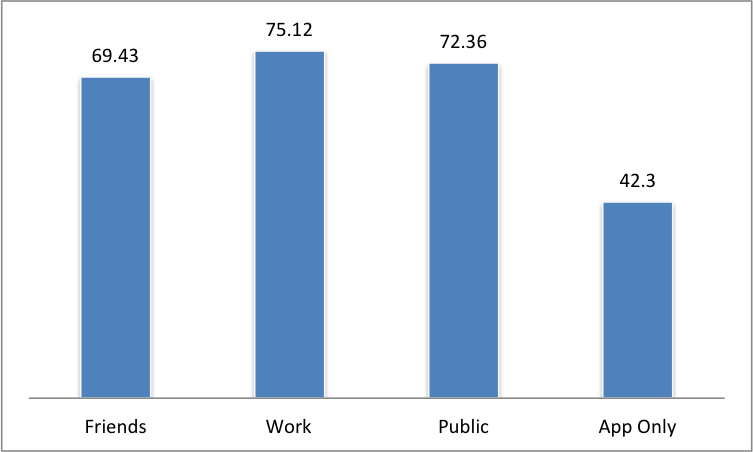
\includegraphics[width=0.5\textwidth]{recipient.png}
%	\caption{(This is a placeholder! TODO: generate a better plot for data recipient)}
%\end{figure}

% LL: I thought this would be better, but then it looked stupid, so I commented it out.

%\begin{table}[t]
%\begin{center}
%\begin{tabular}{|l|c|}
%\hline
%Recipients	& VUR \\
%\hline
%App	& 42.3\% \\
%Friends & 69.4\% \\
%Work & 75.1\% \\
%Public & 72.4\% \\
%\hline
%\end{tabular}
%\caption{VUR rates by recipient.}
%\label{whomVUR}
%\end{center}
%\end{table}

\begin{table}[t]
\begin{center}
\begin{tabular}{|l|r|r|r|r|}
\hline
Recipients	& $\chi^2$ & p-value 	& n & $\phi$ \\
\hline
Work-App	& 564.32 & <0.0001 & 5,085 & 0.111\\
Public-App	& 479.98 & <0.0001 & 5,192 & 0.092\\
Friends-App & 380.00 & <0.0001 & 5,098 & 0.075\\
Friends-Work & 20.37 & <0.0001 & 5,039 & 0.004\\
Friends-Public & 5.35 & <0.0207 & 5,146 & 0.001\\
Work-Public&  5.05 & <0.0246 & 5,133	& 0.001\\
\hline
\end{tabular}
\caption{Results of a chi-square test to examine VUR based on data recipient, across all data points.}
\label{recipient}
\end{center}
\end{table}

%\begin{table}[t]
%\begin{center}
%\begin{tabular}{|l|r|r|r|r|}
%\hline
%Recipients	& $\chi^2$ & p-value 	& n & $\phi$ \\
%\hline
%Work-App	& 42.49	& <0.0001	&	601	&	0.071\\
%Public-App &	48.52	& <0.0001	&		636	&	0.076\\
%Friends-App	& 32.07	& <0.0001	&		609	&	0.053\\
%Friends-Work & 	0.87 &	<0.3517	&	604	&	0.001\\
%Friends-Public	& 1.46 &	<0.2229	&	639	&	0.002\\
%Work-Public &	0.67 &	<0.7956	&		631	&	0.001\\
%\hline
%\end{tabular}
%\caption{Results of a chi-square test to examine VUR based on data recipient, across all data points.}
%\label{recipient}
%\end{center}
%\end{table}

%\begin{table}[t]
%\begin{center}
%\begin{tabular}{| c | c | c | c |}
%Recipients	& $\chi^2$ &	2-tail P &  Effect Size \\
%Work-App	& 564.318 & <0.0001 & 0.111\\
%Public-App	& 479.980 & <0.0001 &  0.092\\
%Friends-App & 380.000 & <0.0001 & 0.075\\
%Friends-Work & 20.365 & <0.0001 &  0.004\\
%Friends-Public & 5.349 & 0.0207 &  0.001\\
%Work-Public&  5.054 & 0.0246 &  0.001\\
%\end{tabular}
%\caption{Chi-Squared test results of the effects of various recipients contributing to VUR.}
%\label{recipient}
%\end{center}
%\end{table}				

%\begin{table}[t]
%\begin{center}
%\begin{tabular}{| l | c |}
%<data> & VUR  \\
%social security number & 98.04\% \\
%a video of you unclothed & 97.44\% \\
%bank account information & 97.10\% \\
%recordings of your work conversations & 96.97\% \\
%an incriminating/embarrassing photo of you & 96.36\% \\
%a photo of you unclothed & 96.30\% \\
%credit card information & 95.92\% \\
%username and password for websites & 95.41\% \\
%a video of you entering in your PIN & 93.91\% \\
%recordings of your phone conversations & 93.88\% \\
%\end{tabular}
%\caption{A table of the top 10 upsetting <data> types, with respect to <recipient> types friends, work, and public.}
%\label{sharedtop10}
%\end{center}
%\end{table}
%
%\begin{table}[t]
%\begin{center}
%\begin{tabular}{| l | c |}
%%starting from #63
%<data> &  VUR  \\
%bank account information & 90.91\% \\
%a video of you unclothed & 90.62\% \\
%social security number  & 88.68\% \\
%video of you entering your PIN & 88.57\% \\
%an incriminating/embarrassing photo of you & 78.05\% \\
%a photo of you unclothed & 77.78\% \\
%a video of you entering a passcode to a door & 75.00\% \\
%when and how much you have sex & 73.08\% \\
%an incriminating/embarrassing video of you & 71.88\% \\
%a random (inward-facing) photo of you at home & 66.67\% \\
%\end{tabular}
%\caption{A table of the top 10 upsetting <data> types, respect to <recipient> app's server only (didn't share it with anyone else).}
%\label{notsharedtop10}
%\end{center}
%\end{table}
%
%\begin{table}[t]
%\begin{center}
%\begin{tabular}{| l | c |}
%%starting from #63
%<data> &  VUR  \\
%your name & 47.25\% \\
%when and how much you exercise & 46.07\% \\
%when you were happy or having fun & 38.10\% \\
%what television shows you watch & 35.96\% \\
%when you are busy or interruptible & 34.34\% \\
%your heart rate & 32.28\% \\
%music from your device & 31.87\% \\
%your age & 29.67\% \\
%the language you speak & 20.95\% \\
%your gender & 16.81\% \\
%\end{tabular}
%\caption{A table of the bottom 10 upsetting <data> types, with respect to <recipient> types friends, work, and public.}
%\label{sharedbottom10}
%\end{center}
%\end{table}
%
%
%\begin{table}[t]
%\begin{center}
%\begin{tabular}{| l | c |}
%%starting from #63
%<data> &  VUR  \\
%when and how much you exercise & 16.67\% \\
%how much you use your phone & 15.79\% \\
%your age & 14.29\% \\
%how much you like the people you interact with & 13.79\% \\
%when, what, and how much you ate & 12.50\% \\
%which television shows you watch & 11.43\% \\
%your gender & 9.52\% \\
%your heart rate & 9.09\% \\
%eye movement patterns (for eye tracking) & 6.98\% \\
%the language you speak & 2.50\% \\
%\end{tabular}
%\caption{A table of the bottom 10 upsetting <data> types, respect to <recipient> app's server only (didn't share it with anyone else).}
%\label{notsharedbottom10}
%\end{center}
%\end{table}
%
%Commonly, bank info, SSN, PIN, embarrassing photo, naked photo, naked video were considered to be highly sensitive. When people perceived that the data would be shared with the app only, the other top five concerns included the passcode to a door, how frequently one has sex, embarrassing videos, and photos at home. When people perceived that the data would be shared with a human audience, their other top concerns were work conversations, credit card information, username and password combinations for websites, and phone conversations. When data is perceived to be shared by an app, people are more concerned with issues of being spied on or tracked, whereas when data is perceived to be shared with an individual, people are concerned more with theft or reputation. 
%
%On the other hand, exercise details, age, tv shows, gender, heart rate, and language were commonly considered to be lease concerning. When people perceived that the data would be shared with the app only, the other indifferent data included phone use, how much one liked the people around, when and what you ate, and eye patterns. When people perceived that the data would be shared with a human audience, the least concerning data included one's name, if one was having fun, music on the device, and if one was busy or interruptible. When sharing with an application, information otherwise considered personal such as phone use, opinions of people, food eaten, or eye patterns were okay to share, since these seem like useful information to improve one's device experience. However, people are not likely to share the same with people, but are more comfortable with sharing data about topics which would come up in causal conversation.


\subsubsection{Data Type}
Irrespective with whom the data was shared or on what device, participants were most concerned about photos/videos, especially if they contain embarrassment, nudity, or financial information. Information which can be used to impersonate the user (i.e. username and password for websites) and invasions of privacy (photos of someone at home) were also considered to be sensitive data. Top and bottom absolute <data> rankings can be seen in Tables ~\ref{top10} and ~\ref{bottom10}. Generally, the most concerning and least concerning data types did not change by recipient. {\color{red} can be said for ~top/bottom5 looking at the recipient lists I commented out; but this isn't too official since we do no stat tests.}

\begin{table}[t]
\begin{center}
\begin{tabular}{| l | c |}

<data> &  VUR  \\
a video of you unclothed & 95.97\% \\
bank account information & 95.91\% \\
social security number & 94.84\% \\
video of you entering in your PIN & 92.67\% \\
a photo of you unclothed & 92.59\% \\
an incriminating/embarrassing photo of you & 91.39\% \\
username and password for websites & 89.55\% \\
credit card information & 88.98\% \\
an incriminating/embarrassing video of you & 88.41\% \\
a random (inward-facing) photo you at home & 87.50\% \\

\end{tabular}
\caption{A table of the top 10 upsetting <data> types, irregardless of recipient or data type.}
\label{top10}
\end{center}
\end{table}

\begin{table}[t]
\begin{center}
\begin{tabular}{| l | c |}
%starting from #63
<data> &  VUR  \\
eye movement patterns (for eye tracking) & 40.51\% \\
when and how much you exercise  & 38.66\% \\
when you are happy or having fun  & 34.51\% \\
which television shows you watch & 30.20\% \\
when you are busy or interruptible  & 29.50\% \\
music from your device  & 28.06\% \\
your heart rate & 27.50\% \\
your age & 24.29\% \\
the language you speak & 15.86\% \\
your gender & 14.91\% \\ 

\end{tabular}
\caption{A table of the bottom 10 upsetting <data> types, irregardless of recipient or data type.}
\label{bottom10}
\end{center}
\end{table}

A statistical analysis regarding the significance and confidence of <data> types with respect to all 72 was not performed due to the space constraints of the paper. We do consider all <data> categories in our statistical model, which provides an analysis of what factors had contributed to the perceived severity of a particular situation. 

\subsubsection{Device Type}
Participants had unique VUR rates for situations only differing in the device. Our participants had a 70.23\% VUR when asked about wearables devices and 40.62\% VUR when asked about smartphones.The VUR rates for both devices for all 5 quesions are in table ~\ref{deviceVUR}. However, the effect the device has on the VUR is not considered to be statistically significant (see Table ~\ref{betweendevice}). Additionally, there is no statistically significant difference between how people reacted in a given situation; although, participants were statistically significantly upset in Q2.  The aforementioned results are only with respect to between subjects analysis, where answers are from participants who received either only the wearables or smartphone version of the 5 questions. There were too few instances where a participant got both versions of questions (34 in total for all 5 questions), to be able to perform a within-subjects analysis. 

\begin{table}%[h]
\begin{center}
\begin{tabular}{| c | c | c |}
 Question &  Wearable VUR & Smartphone VUR \\
 All & 70.23\% & 40.62\%\\
Q1 & 14.81\%  &  6.13\%\\
Q2 & 44.11\%  &  19.85\%\\
Q3 & 87.09\%  &  58.44\%\\
Q4 & 52.77\%  & 55.79\%\\
Q5 & 86.49\%  &  91.82\%\\ 
\end{tabular}
\caption{A table of the bottom 10 upsetting <data> types, respect to <recipient> app's server only (didn't share it with anyone else).}
\label{deviceVUR}
\end{center}
\end{table}

\begin{table}%[h]
\begin{center}
\begin{tabular}{| c | c | c | c |}
%Question & Chi^2 &	2-tail P &	Sig?	 & n	& effect size\\
%All	2.814	0.1395	No		3589		0.001\\
%Q1	2.500	0.1139	No		714		0.004\\
%Q2	17.333	<0.0001	Yes		708		0.024\\
%Q3	0.020	0.8886	No		699		0.000\\
%Q4	1.426	0.2324	No		731		0.002\\
%Q5	1.611		0.2043	No		710		0.002\\
Question & $\chi^2$ &	2-tail P & Effect Size\\
All & 2.814 & 0.1395 & 0.001\\
Q1 & 2.500 & 0.1139 & 0.004\\
Q2 & 17.333 & <0.0001 & 0.024\\
Q3 & 0.020 & 0.8886 & 0.000\\
Q4 & 1.426 & 0.2324 & 0.002\\
Q5 & 1.611 & 0.2043 & 0.002\\
\end{tabular}
\caption{Results of the effects of <device> type contributing to VUR. Values are Chi-Square test results for between-subjects comparisons for participants who received one question, but not the other.}
\label{betweendevice}
\end{center}
\end{table}
						
%\begin{table}%[h]
%\begin{center}
%\begin{tabular}{| c | c | c | c |}
%Question & $\chi^2$ &	2-tail P & Effect Size \\
%All & 0.444  & 0.505 & 0.006\\
%Q1 & 0 & 1 & 0 \\
%Q2 & 0 & 1 & 0\\
%Q3 & 0 & 1 & 0\\
%Q4 & 0 & 1 & 0\\
%Q5 & 0 & 1 & 0\\
%\end{tabular}
%\caption{Results of the effects of <device> type contributing to VUR. Values are McNeamar's test results for within-subjects comparisons for participants who received both questions.}
%\label{withindevice}
%\end{center}
%\end{table}

%For the between-subjects comparison (i.e., participants who received one question, but not the other), you can do either a chi-square test or Fisher's exact test. Both use a 2 x 2 contingency matrix (i.e., rows are outcomes---upset or not---and columns are conditions---wearable or smartphone). The way to choose between the two tests is based on sample size, generally you use chi-square when there are more than 10-20 samples per cell in the table, but using either is just as valid. For the within-subjects comparisons (i.e., participants received both questions), you would do McNemar's test; which is the within-subjects version of the chi-square test. 

\subsubsection{Regression Model} 
Introduce the model and what was considered in the model. Serge can probably do this better. Talk about which factors mattered, and how much, and also interesting statistics we found, if any. Also, correlations with demographics here as well! 

\subsection{Risk and Benefit Rankings} 
When assessing new technologies, participants generally had rated the technologies similarly, considering them low risk and low benefit (see figure \ref{fig:techplot}). We suspect that these similar assessments are because most are not consciously aware of the possibilities of these technologies or how they are being used today. A list of the ranking of most risky and most beneficial technologies can be see in appendix \ref{sec:techrank}; the most risky and most beneficial technologies reveals the list of most familiar technologies for the average user (internet, laptops, email, smartphones, etc.). 

{\color{red} can you redo the graph for figure ~\ref{fig:techplot}? I trust your judgement on how it should look and what to emphasize.}

\begin{figure}
	\centering
	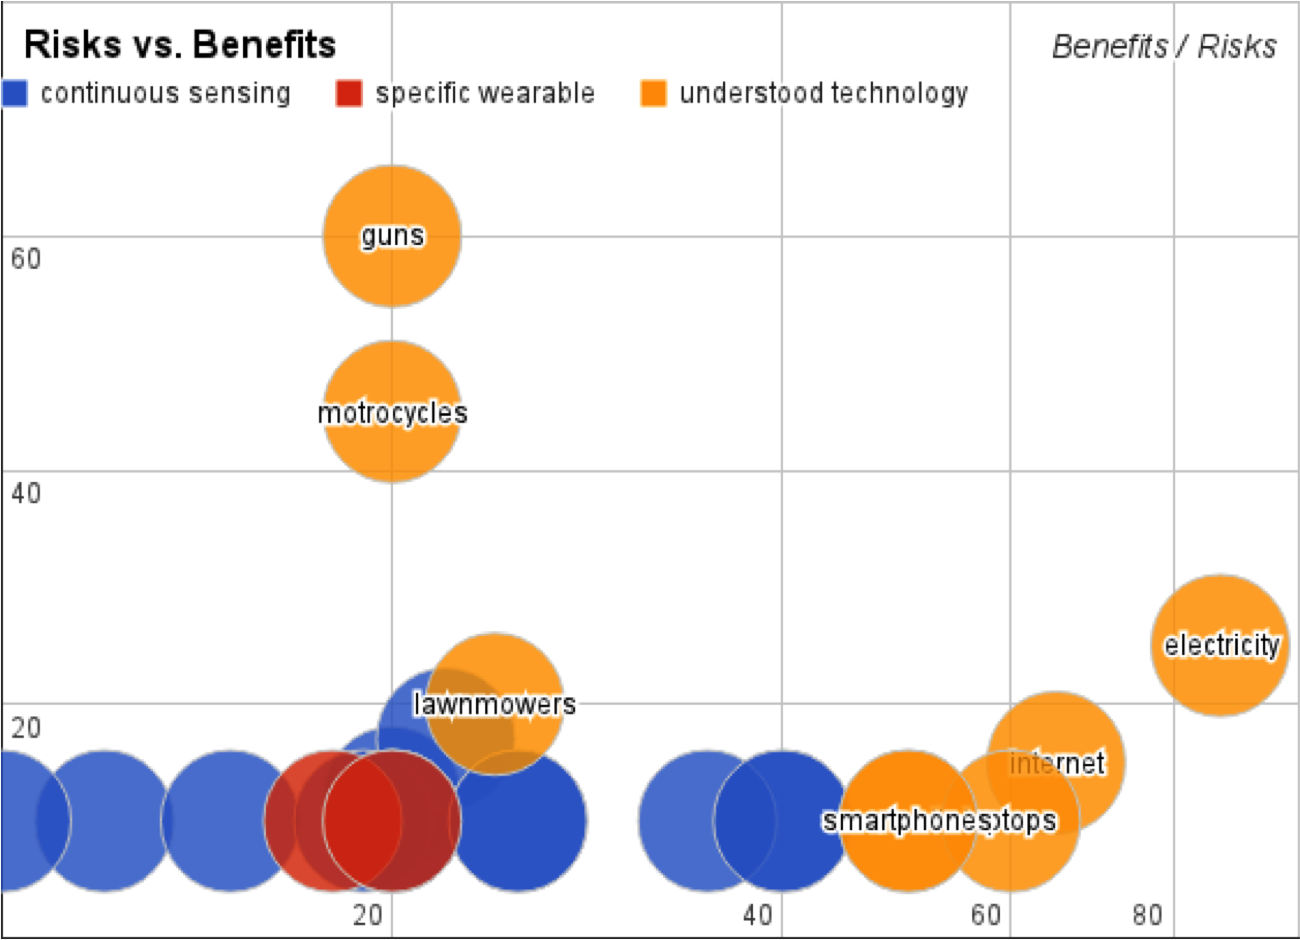
\includegraphics[width=0.5\textwidth]{techplot.png}
	\caption{(This is a placeholder! TODO: generate a better plot; take out the specific wearables too.)}
	\label{fig:techplot}
\end{figure}

Notably, technologies perceived to be beneficial include location tracking and heart rate detection. Again, we believe this is the result of exposure people have to these technologies--most people use GPS or other location-based applications on their smart phones and fitness trackers are the most popular type of wearable device. Technologies considered to be risky, such as a discrete camera and facial detection, seemed to be based on media exposure or general aversion to privacy invasion. However, people are becoming increasingly aware of such risks and are comparing these risks of privacy invasion to real physical risks--for instance, the capacity for facial detection on a wearable device is perceived to be almost as risky as interacting with a physical lawnmower. It is fair to say that, these assessments of the most risky or beneficial technologies may not be the most accurate, but do reflect the exposure of various technologies to the general public and also prove that people do perceive risks in a real way related to these technologies. 

\subsection{Perceived Concerns for Wearable Devices}
So far, participants had responded to questions regarding specific scenarios or assessed technologies presented to them. For completeness of the survey, we also wanted to capture the participants' general reactions to wearable devices as a whole. To do this, we asked the participants an open-ended question regarding the most likely risks associated with owning and interacting with wearable devices.

\textit{What do you think are the most likely risks associated with wearable devices?}\\[-.5cm]

This question was asked along with the demographics questions, near the end of the survey, but before any IUIPC questions regarding privacy, to avoid biasing. The participants were presented with a blank box to write in, with no character limit to their open-ended responses. 

Without any doubt, the open-ended responses state that the most common concern for owning and interacting with wearable devices for the average user is the \textit{possible loss of privacy}. This top concern surpassed all other concerns by about an order of magnitude or more:

%% I EDITED THESE NUMBERS for 17 year old

\begin{table}[h]
\begin{center}
\begin{tabular}{lll}

Concern &  Responses &  Frequency   \\
Privacy & 452 & 25.32\% \\
Being Unaware & 275 & 15.40\ \\
%Unaware Use & 167 & (9.36\%)\\
%Unaware Collection & 64 & (3.59\%)\\
%Unaware Access & 44 & (2.46\%)\\
Health Risk & 191 & 10.70\%\\
Safety & 185 & 10.42\%\\
Financial Cost & 151 & 8.46\%\\
Security &	144 & 8.07\%\\
Social Impact &	157 & 8.80\%\\
Accidental Sharing &	69 & 3.87\%\\
Miscellaneous &	57 & 3.19\%\\
None	& 51 & 2.86\%\\
Social Stigma &	39 & 2.18\%\\
False Information & 33 & 1.85\%\\
Don't know & 31 & 1.74\%\\
Aesthetics 	& 19 & 1.06\%\\
Don't care 	& 11 & 0.62\%\\

\end{tabular}
\caption{A table listing the self-reported most common risks associated with owning a wearable device.}
\label{open-responses}
\end{center}
\end{table}

Other significant secondary concerns included being unaware of what the device is collecting, doing, or which information it is using (Being Unaware), long-term health effects caused from wearing the device such as cancer from emf waves (Health), safety hazards from wearing the device such as battery burns or distractions causing car accidents (Safety), the high financial cost of buying, replacing, or caring for the device (Financial),  information compromise (Security), and resulting changes in social behaviors, such as dependencies on devices or spending less time with loved ones (Social Impact). Refer people to the appendix \ref{sec:coding} for detailed information on coding labels. 

%%%%%%%%%%%%%%%%%%%

\section{Discussion}
We take this section to discuss complementary future research directions in fields of privacy, ubiquitous computing, and user studies, along with specific limitations of this survey. 

\subsection{Future Research Directions}

Our survey shows that photos, videos, and textual information is generally considered to be very sensitive. Various systems which can detect and take actions for sensitive objects in photos and videos will be critical as wearables and other devices become more ubiquitous. We also show that users are significantly more willing to offer certain data if it will only be shared with the application; and additionally, that users consider privacy as their number-one concern. Research in effective sandboxing and other software protections, effective notifications, and usable indicators are encouraged at this time. Lastly, exploratory research investigating user-reported concerns, are relevant--especially the social impact of wearable devices, measurement of inaccuracy of sensor readings presented by wearables, and rate of accidental information sharing. 

\subsection{Limitations}
One of the main limitations of this work is that our participants might not have interest, or an accurate idea, of wearables and their capabilities. 83\% of our participants reported that they do not own a wearable device, but at this time, about ~15\% of the general population own and use wearable devices \cite{Nilsen,WearableStatNews}, so our study is reflective of the status quo. We believed that getting a representative survey base was a useful endeavor, although we could have easily recruited only wearable device owners or people specifically interested in wearables. However, that will also have its own bias and limitations as well, since they would not reflect the general population. We expect user perceptions to change as rapidly as wearable technologies and the rate of adoption change. 

%The survey was constructed in a way to randomize the order of the particular sets of questions participants saw, except for the open-ended question, which was always near the end of the survey, asked along with the demographics. For this reason, people were heavily primed for the open-ended question. However, this question was always shown before the IUIPC questions, so our results on privacy being the top concern isn't because of the bias from the privacy index. The intent of the open-ended question  was more to get a sense of what people were concerned of, and we believe the results do reflect their actual concerns, but with a bit more clarity, since the participants were already thinking about such risks related to wearables. 

%(REDO, Should I even say this?) I messed up that motorcycle question. I wish I actually had a calibration point for high risk high benefit for the Fischoff technology assessment questions. But well, none of the new technologies fit that description so we didn't really need it critically. 

%%%%%%%%%%%%%%%%%%%

\section{Conclusion}

We surveyed 2,250 internet users to determine what contributes to a violation of privacy or security, which technologies are risky, and what users think are the biggest risk for operating wearable devices. Participants rated how upset they would be if 304 situations occurred, assessed the risk and benefit for 20 new technologies, and gave open-ended responses to express their concerns. We provide insight into how much and why data, recipient, and device contribute to users' perception of a situation, calibrate answers with existing smartphone literature, and provide a regression model. An assessment of a range of new technologies shows that users perceive new technologies to be low-risk and low-benefit, but we suspect this is due to limited exposure that an average person has with wearables techology. We also state what users perceived as the most significant concerns with respect to wearable devices. We conclude by discussing future research directions in the wearables and user study space. 

%\end{document}  % This is where a 'short' article might terminate

%ACKNOWLEDGMENTS are optional
\section{Research Ethics} 
We received advance approval from University of California, Berkeley's Institutional Review Board to perform this user study. Survey data was collected in an anonymous manner. Although the focus group was not conducted in an anonymous manner, participants were not asked to offer any confidential or sensitive information. 

\section{Acknowledgments}
The authors would like to thank The National Science Foundation's Graduate Research Fellowships Program (NSF GRFP), and the Intel Science and Technology Center for Secure Computing (also known as  Secure Computing Research for Users' Benefit, SCRUB), for the support of this research. Inspiration for this work emerged out of fruitful discussions at the Berkeley Laboratory for Usable and Experimental Security (BLUES) meetings. Many thanks go out to the many generous colleagues who have provided feedback and encouragement.


%%%%%%%%%%%%%%%%%%%
%%%            BIB & ACKS          %%%
%%%%%%%%%%%%%%%%%%%

% The following two commands are all you need in the initial runs of your .tex file to produce the bib
%  and remember to run: latex bibtex latex latex to resolve all references

\bibliographystyle{abbrv}
\bibliography{wearables_survey}  % wearables_survey.bib is the name of the Bibliography


%APPENDICES are optional
%\balancecolumns
\appendix
%Appendix A
\section{Fischhoff Prompts}
\label{sec:prompt} 

\textit{We would like to ask you to rate the <risks/benefits> associated with each of the following technologies.}

{\bf Risks:} \textit{Consider all types of risks: the risk of physical harm or death, the risk to others or bystanders, the financial cost of the technology, any distress caused by the technology, what the consequences would be if the technology was misused, any impact on the public, work, or personal life, and other considerations. (e.g. for electricity, consider the risk of electrocution, the pollution caused by coal, the risk that miners need to take to mine the coal, the cost to build the infrastructure to deliver electricity, etc.) Give a global estimate over a long period of time (say, a year) of both intangible and tangible risks.} \\[-.6cm]

\textit{Do not consider the costs or risks associated with these items. It is true, for example, that sometimes swimmers can drown. But evaluating such risks is not your present job. Your job is to assess the gross benefits, not the net benefits which remain after the costs and risks are subtracted out.} \\[-.6cm]

\textit{Please rate the following technologies below with a number. We know that this might be a bit hard to do, but please try to be as accurate as possible, adjusting the numbers until they feel they are right for you. Start with the least risky technology at 10 and assign higher numbers for the more risky technologies. (For instance, a technology rated 14 is half as risky as a technology rated 28.)}

{\bf Benefits:} \textit{Consider all types of benefits: how many jobs are created, how much money is generated directly or indirectly, how much enjoyment is brought to people, how much a contribution is made to the people's health and welfare, what this technology promotes, and so on. (e.g. for swimming, consider the manufacture and sale of swimsuits, the time spent exercising, the social interactions during swimming, and the sport created around the activity.) Give a global estimate over a long period of time (say, a year) of both intangible and tangible benefits.} \\[-.6cm]

\textit{Do not consider the costs or benefits associated with these items. It is true, for example, that electricity also creates a market for home appliances. But evaluating such benefits is not your present job. Your job is to assess the gross risks, not the net risks which remain after the costs and risks are subtracted out.} \\[-.6cm]

\textit{Please rate the following technologies below with a number. We know that this might be a bit hard to do, but please try to be as accurate as possible, adjusting the numbers until they feel they are right for you. Start with the least beneficial technology at 10 and assign higher numbers for the more beneficial technologies. (For instance, a technology rated 34 is twice as beneficial as a technology rated 17.)}


%\section{Risk and Benefit Rankings}
%\label{sec:techrank}
%
%BENEFIT: 
%
%technology 	median	25\%		75\% \\
%electricity	87	50	100\\
%internet	65	45	100\\
%laptops	60	40	80\\
%email	50	30	75\\
%smartphones	50	32.5	75\\
%location tracking	40	20	67.5\\
%heart rate detection	40	28	62.5\\
%language detection	35	15	60\\
%voice recognition	25	15	40\\
%speech to text	25	15	36.25\\
%lawnmowers	24	15	40\\
%facial recognition	22	13	40\\
%guns	20	10	30\\
%motrocycles	20	12	40\\
%voice based emotion detection	20	10	30\\
%facial detection	20	10	32\\
%discrete camera	20	15	30\\
%smartwatches	20	10	32.5\\
%google glass	20	12	40\\
%fitness trackers	19	10	30\\
%cubetastic	18	10	30\\
%discrete microphone	15	10	20\\
%age detection	12	10	21\\
%gender detection	10	10	15
%
%RISK: 
%
%technology 	median	25\%		75\%\\
%guns	60	40	80\\
%motrocycles	45	27	70\\
%electricity	25	15	40\\
%lawnmowers	20	12	30\\
%facial recognition	17	12.5	30\\
%internet	15	10	30\\
%discrete camera	12	10	30\\
%location tracking	10	10	20\\
%age detection	10	10	15\\
%gender detection	10	10	12\\
%language detection	10	10	10\\
%voice based emotion detection	10	10	15\\
%facial detection	10	10	25\\
%voice recognition	10	10	15\\
%heart rate detection	10	10	10\\
%email	10	10	16\\
%speech to text	10	10	10\\
%discrete microphone	10	10	20\\
%smartphones	10	10	19\\
%laptops	10	10	15\\
%fitness trackers	10	10	10\\
%smartwatches	10	10	10\\
%google glass	10	10	20\\
%cubetastic	10	10	30

%\section{Coding Label Definitions}
%\label{sec:coding}
%
%Privacy: ``privacy,'' revealing personal information, spying. \\
%Security:  ``security,'' compromise, malware, hacking. \\
%GPS tracking: ``location,'' ``GPS,'' being monitored. 
%
%Unaware use: using data without permission or in a different way than understood by user. \\
%Unaware collection: collecting data without permission. \\
%Unaware access: disclosure of data without permission. \\
%False information: inaccurate or maliciously false data.
%
%Health Risk: radiation, cancer, or long-term effects.\\
%Safety: distractions causing car crashes or injuries, mugging or violence because of the device, injuries from device malfunctions (battery burns).\\
%Discomfort: eye strain, headache, obscured vision, irritation. \\
%Financial cost: getting ripped off by buying the device or device accessories, having to buy another device when broken or stolen, financial compromise caused by device. \\
%Theft: the device getting stolen. 
%
%Social Impact: dependency, distance from friends and family, changes in decision making, social changes, etc. \\
%Social Stigma: judgment, hate, or bystander discomfort.\\ 
%Aesthetics: fashion, the device being ugly, mentions of not looking cool/dorky. 
%
%Miscellaneous: odd comments, uncommon concerns. \\
%None: ``None,'' no threat, perceiving no big concerns \\
%Don't know: ``do not know,'' hinting at confusion \\
%Don't care: `` do not care,'' nonchalant answers 


%\section{Detailed Tech Rankings}

\balancecolumns

% That's all folks!
\end{document}
\\